\begin{figure}
\centering
\begin{subfigure}{.15\textwidth}
  \centering
  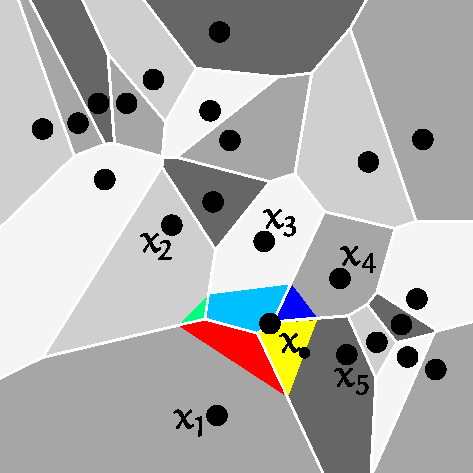
\includegraphics[width=\linewidth]{voronoi1.pdf}
  \caption{Inserting a point.}
\end{subfigure}\hfill
\begin{subfigure}{.15\textwidth}
  \centering
  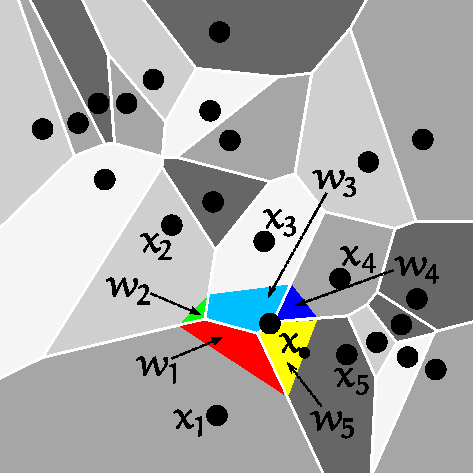
\includegraphics[width=\linewidth]{voronoi2.pdf}
  \caption{Cells $\Vor(x_i)$.}
\end{subfigure}\hfill
\begin{subfigure}{.15\textwidth}
  \centering
  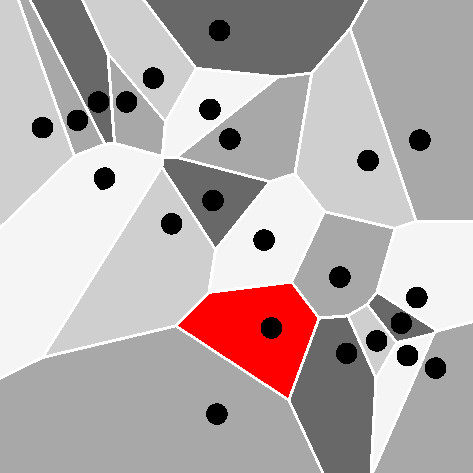
\includegraphics[width=\linewidth]{voronoi3.pdf}
  \caption{$\text{dgm}_{\Vor}(X \cup x_\bullet)$.}
\end{subfigure}
\caption{(a) Clipped tesselation. For other manifolds the curvature should be considered. (b) Tesselation with added point creates a new Voronoi region \textit{stealing} area from the neighboring regions. (c) The determined weights by the fractional amount of occupied area. (d) Tesselation with added point.}
\label{fig:voronoi}
\end{figure}
